\documentclass[11pt,a4paper]{article}

\usepackage[margin=2.0cm]{geometry}
\usepackage[T1]{fontenc}
\usepackage[utf8]{inputenc}
\usepackage{microtype}
\usepackage{lmodern}
\usepackage{booktabs}
\usepackage{array}
\usepackage{enumitem}
\usepackage{hyperref}
\usepackage{xcolor}
\usepackage{amsmath}
\usepackage{amssymb}
\usepackage{titlesec}
\usepackage{caption}
\usepackage{graphicx}
\usepackage{float}
\usepackage{subcaption}

\graphicspath{{../results/figures/}}

\hypersetup{
  colorlinks=true,
  linkcolor=black,
  urlcolor=blue!60!black,
  citecolor=blue!60!black,
  pdftitle={CENG 463 Progress Report -- Probabilistic Forecasting with Anomaly Injection}
}

\titlespacing*{\section}{0pt}{0.9ex}{0.9ex}
\titlespacing*{\subsection}{0pt}{0.7ex}{0.3ex}
\setlist{topsep=1pt,itemsep=0pt,parsep=0pt}
\setlength{\parskip}{2pt}
\setlength{\textfloatsep}{6pt}
\setlength{\intextsep}{6pt}
\setlength{\abovecaptionskip}{3pt}
\setlength{\belowcaptionskip}{0pt}
\sloppy

\begin{document}

\begin{center}
{\Large\bfseries Probabilistic Forecasting with Anomaly Injection}\\[2pt]
{\large CENG 463 -- Introduction to Machine Learning -- Progress Report}\\[2pt]
\.{I}zmir Institute of Technology, Spring 2026\\[2pt]
Instructor: Prof. Dr. Aytu\u{g} Onan\\[2pt]
Group Members: Ozan Erdo\u{g}an, Student No.\ 290201102
\end{center}

\section{Problem Definition}

\paragraph{Task.}
I work with a multivariate weather time series
$\{x_{t}\}_{t=1}^{T}$ where each $x_t \in \mathbb{R}^{14}$ is a vector of
hourly meteorological variables. The model takes the past $L=168$ hours
(one week) of context and predicts the next $H=24$ hourly air-temperature
values. Two model families are compared. \emph{Deterministic} models
output a single point forecast in $\mathbb{R}^{H}$. \emph{Probabilistic}
models output a predictive distribution
$p(y_{t+1:t+H} \mid x_{t-L+1:t})$ summarised by quantiles and
prediction-interval coverage. After in-distribution evaluation, every
model is re-evaluated under controlled \emph{anomaly injection}: spikes,
contextual outliers, level shifts, and FGSM-style perturbations are
added to the test inputs at varying intensity. The question I want to
answer is whether probabilistic models lose accuracy more slowly than
deterministic ones, and whether their uncertainty actually rises around
the injected anomalies.

\paragraph{Importance.}
Real weather forecasting systems often receive imperfect inputs due to sensor faults, missing updates, or unusual local conditions. Therefore, clean-data accuracy alone is not enough to judge whether a model is reliable in practice. This project evaluates how forecasting models behave under controlled input anomalies. This is important because useful uncertainty estimates can help users decide when a forecast should be trusted or treated with caution.

\paragraph{Dataset.}
The project uses the Jena Climate dataset, a multivariate weather time-series dataset containing meteorological variables such as air temperature, pressure, humidity, and wind-related measurements. The data is resampled to hourly frequency.

\paragraph{Inputs / outputs.}
\textbf{Input:} a 168-hour context window of 14 meteorological variables. \textbf{Output:} the next 24 hourly air-temperature values, either as a point forecast for deterministic models or as a predictive distribution for probabilistic models.

\paragraph{Task family.}
This project is a multistep time-series forecasting task with an additional robustness evaluation component. The main goal is to predict future temperature values from past weather observations. The anomaly-injection part extends the task by testing how stable the models remain when the input data becomes abnormal.

\paragraph{Challenges.}
Scaling these forecasts over a 24-hour horizon introduces several technical difficulties. Errors can accumulate across future steps, especially in autoregressive models. Probabilistic models must produce not only accurate forecasts but also well-calibrated uncertainty estimates, so their prediction intervals should contain the true values at the expected rate. Anomaly injection must also be designed carefully: very small anomalies may have little effect, while unrealistic anomalies can make the task trivial. Therefore, the evaluation must consider both clean-data accuracy and robustness under abnormal inputs.

\section{Dataset and Preprocessing Status}

\paragraph{Dataset.}
Jena Climate 2009--2016, recorded at the Max Planck
Institute for Biogeochemistry in Jena, Germany. The raw archive holds
$420{,}551$ observations spaced 10 minutes apart, with 14 variables
covering pressure, temperature, dew point, humidity (relative,
specific, and as water-vapour concentration), the saturation /
actual / deficit family of vapour pressures, air density, wind speed,
maximum gust, and wind direction.

\paragraph{Source and acquisition.}
The dataset is hosted on the
TensorFlow CDN. \texttt{scripts/download\_data.py} downloads the
$\sim$\,13~MB zip, unpacks it, and writes the cleaned hourly version
to \texttt{data/processed/jena\_hourly.parquet}.

\paragraph{Preprocessing performed.}

\begin{itemize}
  \item Parsed the timestamps and resampled to hourly means: this turns
        the raw $420{,}551$ rows into $70{,}128$ hourly rows.
  \item The raw wind-speed columns occasionally store large negative
        sentinel values; these were turned into NaN before averaging.
  \item Around 2014-09-24 / 2014-09-25, the station logged no data for roughly three        days. This gap is filled using time-aware linear interpolation, with forward/       backward filling at the edges, so the processed hourly series contains no           missing values.
  \item The raw archive ends at 2016-12-31 23:50, which falls into the
        2017-01-01 hour bucket; that incomplete bucket was dropped, and
        the series ends cleanly at 2016-12-31 23:00.
  \item Stored as Parquet so reload is fast.
\end{itemize}
After these preprocessing steps, the dataset is ready to be split and converted into forecasting windows for model experiments.

\begin{figure}[H]
\centering
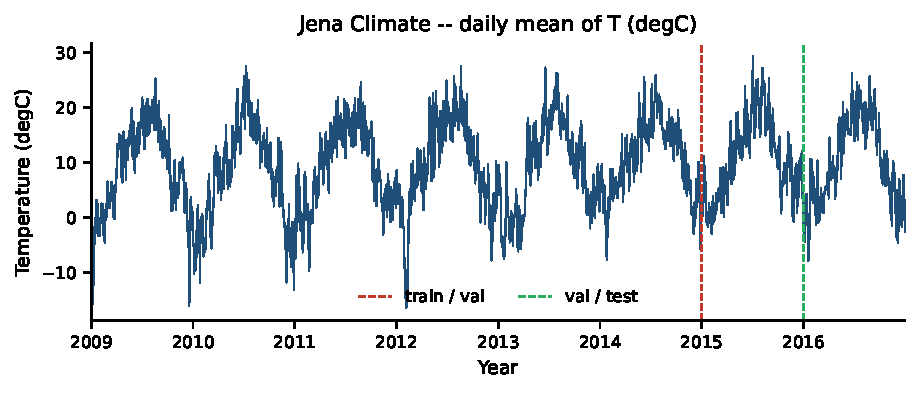
\includegraphics[width=0.86\linewidth]{jena_series_split.pdf}
\caption{Daily-mean temperature across the full record, with the
chronological train/validation/test boundaries (red: end of train,
green: end of validation). Yearly seasonality is the dominant signal,
and a mild upward trend is visible across years.}
\label{fig:series-split}
\end{figure}

\paragraph{Splits (chronological, deterministic).}
\begin{center}
\begin{tabular}{lll}
\toprule
Split & Range & Hours \\
\midrule
Train & 2009-01-01 -- 2014-12-31 & $\sim$\,52{,}584 \\
Validation & 2015-01-01 -- 2015-12-31 & $\sim$\,8{,}760 \\
Test & 2016-01-01 -- 2016-12-31 & $\sim$\,8{,}784 \\
\bottomrule
\end{tabular}
\end{center}

\paragraph{Target.}
The air-temperature channel \texttt{T (degC)}, with a
range of roughly $-25$ to $+38$\,$^{\circ}$C across the record. The
remaining 13 channels become exogenous covariates in later phases.

\paragraph{Standardisation and windowing.}
The target channel is standardised using statistics fitted on the training split only, and predictions are converted back to degrees before metric computation. For the LSTM baseline, sliding windows are constructed with lookback $L=168$ and horizon $H=24$. Training windows use stride 1, while validation and test windows use stride $H$ to reduce overlap. Rolling-origin baselines such as ARIMA and seasonal naive forecasting are evaluated separately.

\paragraph{Issues encountered and resolved.}
An earlier hourly version still contained missing values from the September 2014 outage, which caused failures during metric computation. This was fixed by applying time-aware linear interpolation followed by forward/backward filling at the edges. The incomplete final hourly bucket was also removed so that the processed series ends cleanly at 2016-12-31 23:00. No class imbalance issue exists because the target is continuous air temperature rather than a discrete class label.

\paragraph{Preprocessing steps completed.}
After these preprocessing steps, the dataset has been downloaded, cleaned, resampled to hourly frequency, saved as Parquet, split chronologically, and prepared for baseline model experiments.

\section{Literature Review Progress}

\paragraph{Deterministic forecasting baselines.}
Hyndman and Athanasopoulos (\emph{Forecasting: Principles and Practice}, 2021)
present seasonal naive forecasting and ARIMA as standard reference methods for
time-series forecasting. This supports the use of a seasonal naive model as a
simple sanity-check baseline for hourly temperature, where daily seasonality is
strong, and ARIMA as a classical statistical baseline. For the neural
deterministic baseline, Hochreiter and Schmidhuber (1997) introduced the LSTM
architecture, which is widely used for sequential data because it can model
longer temporal dependencies than a simple recurrent network. In this project,
the LSTM uses the same lookback and horizon setting as the later probabilistic
models, giving a stronger deterministic reference point before evaluating
DeepAR and the quantile-based Transformer.

\paragraph{Probabilistic forecasting.}
Salinas et al.\ (\emph{DeepAR}, 2020) propose an autoregressive RNN that,
at every step, outputs the parameters of a likelihood such as a Gaussian or
Negative Binomial distribution and is trained by maximizing the likelihood.
This motivates DeepAR as the parametric probabilistic baseline for this
project. Wen et al.\ (\emph{MQ-RNN}, 2017) take a different route: a
multi-quantile forecasting head trained with the pinball loss, without making
a fixed distributional assumption. This motivates the quantile-based
Transformer baseline. Zhou et al.\ (\emph{Informer}, 2021) and Wu et al.\
(\emph{Autoformer}, 2021) are Transformer architectures specialized for
long-horizon forecasting. Their experimental setup helps guide the choice of
lookback, horizon, and channel handling so that the LSTM and Transformer
models are evaluated under a consistent forecasting protocol.

\paragraph{Adversarial / anomaly evaluation.}
Goodfellow et al.\ (FGSM, 2015) and Madry et al.\ (PGD, 2018) provide the
main background for gradient-based input perturbations. Although these methods
were originally developed for adversarial attacks on classifiers, their
perturbation-budget idea and $\ell_{\infty}$-norm constraint are useful for
this project as a controlled way to define bounded input noise. In the planned
anomaly-injection stage, an FGSM-style setting will be used as one type of
input perturbation rather than as a full classifier attack.

For non-adversarial anomalies, Blázquez-García et al.\ (2021) summarize common
time-series anomaly types such as point, contextual, and collective anomalies.
This taxonomy fits the planned injection types in this project, including
spikes, contextual outliers, and level shifts. Finally, Gneiting and Raftery
(2007) motivates the use of proper scoring rules such as CRPS, which is
important because the probabilistic models must be evaluated not only by point
error but also by the quality of their predictive distributions.

\paragraph{Methodological implications.}
The reading suggests three concrete decisions. (1)~Use seasonal naive, ARIMA,
and LSTM as deterministic baselines before comparing against probabilistic
models. (2)~Use DeepAR as the parametric probabilistic model and a
quantile-based Transformer as the non-parametric probabilistic model.
(3)~Evaluate the models not only with MAE and RMSE, but also with CRPS,
pinball loss, prediction-interval coverage probability (PICP), and mean
interval score (MIS). This allows the project to discuss both forecasting
accuracy and uncertainty quality under clean and anomalous inputs.

\section{Baseline Models}

At this checkpoint, all three selected baseline models are implemented
and can produce evaluation metrics. The numerical results are reported
in the following section.

\paragraph{Baseline selection rationale.}
\begin{itemize}
  \item \textbf{Naive Seasonal} with $S=24$. This is the simplest
        baseline for an hourly series with a strong daily cycle: the
        forecast for each hour is the value from the same hour on the
        previous day. It serves as a sanity-check baseline that learned
        models should be able to beat.

  \item \textbf{ARIMA}$(2,1,2)$ with rolling-origin refitting. This is
        included as a classical linear statistical forecasting baseline.
        The order is fixed for now; order selection via auto-ARIMA is a
        Phase~2 item. I keep it non-seasonal in this phase so that the
        seasonal naive model separately captures the daily-cycle effect,
        while ARIMA provides a lightweight statistical reference point.

  \item \textbf{LSTM} ($L=168$, $H=24$, hidden $64$, $2$ layers,
        dropout $0.1$, MSE loss, Adam $10^{-3}$, $8$ epochs). This is a
        small deterministic neural baseline. Its capacity is kept
        intentionally modest because the later anomaly experiments require
        a fast retraining loop, and the comparison should focus on
        deterministic versus probabilistic behaviour rather than simply
        on the effect of using a larger network.
\end{itemize}

\paragraph{Status.}
All three baselines are implemented under \texttt{src/baselines/} and
are runnable from \texttt{scripts/run\_*.py}. Each script writes a JSON
file under \texttt{results/}. ARIMA refits every $50$ origins on a
moving 8000-sample window so that the rolling evaluation finishes in a
reasonable time on a laptop.

\paragraph{Implementation issues.}
Two implementation issues appeared during baseline evaluation. First,
an earlier hourly Parquet file still contained missing values from the
September~2014 outage, which caused the metric computation to fail. This
was fixed in preprocessing by applying time-aware interpolation followed
by forward/backward filling at the edges. Second, MAPE produced
misleadingly large values, often above $100\%$, for every model. This
happens because air temperature in Celsius can cross or approach zero in
winter, making the relative-error denominator very small. Switching to
Kelvin would only hide the issue: standardised or differenced models are
invariant to a constant offset, so MAE and RMSE remain unchanged by the
unit change, while MAPE changes artificially. Therefore, I keep MAE and
RMSE as the primary metrics here and will add sMAPE and MASE in Phase~2.

\section{Initial Experimental Results}

The numbers below are on the held-out 2016 test split, target
\texttt{T (degC)}, horizon $H=24$, predictions in original units.
ARIMA is evaluated on the first $30$ days of test using rolling origins
because of refit cost; the other two baselines run over the full test
split. The number of predictions differs across models because the LSTM
is evaluated on non-overlapping 24-hour windows, while the rolling
baselines generate forecasts over more origins.

\begin{center}
\captionof{table}{Phase-1 baseline forecasting results on Jena Climate.
Lower is better.}
\begin{tabular}{lrrrl}
\toprule
Model & RMSE\,($^\circ$C) & MAE\,($^\circ$C) & \#preds & Status \\
\midrule
Naive Seasonal ($S{=}24$) & $3.21$ & $2.44$ & $209{,}688$ & implemented \\
ARIMA$(2,1,2)$            & $4.50$ & $3.64$ & $16{,}728$  & implemented \\
LSTM ($L{=}168, H{=}24$, h$=64$, 2 layers) & $\mathbf{2.43}$ & $\mathbf{1.80}$ & $8{,}616$ & implemented \\
\bottomrule
\end{tabular}
\end{center}

\begin{figure}[H]
\centering
\begin{subfigure}[t]{0.46\linewidth}
\centering
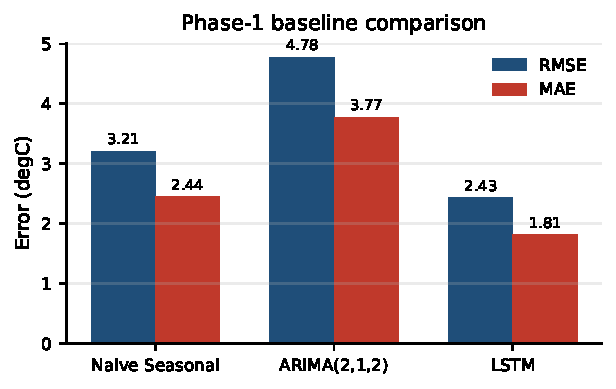
\includegraphics[width=\linewidth]{baseline_comparison.pdf}
\caption{Aggregate RMSE / MAE per baseline.}
\label{fig:bars}
\end{subfigure}\hfill
\begin{subfigure}[t]{0.50\linewidth}
\centering
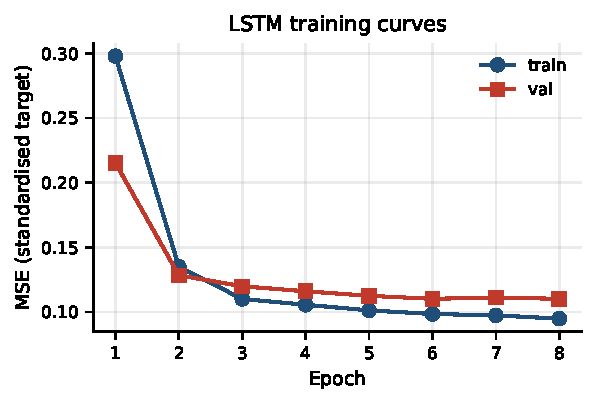
\includegraphics[width=\linewidth]{lstm_loss_curves.pdf}
\caption{LSTM training and validation loss (8 epochs).}
\label{fig:loss}
\end{subfigure}
\caption{Phase-1 baseline summary. The bar chart on the left makes the
model ordering visible at a glance; the loss curves on the right suggest
that the LSTM is not overfitting within eight-epoch.}
\label{fig:summary}
\end{figure}

\begin{figure}[H]
\centering
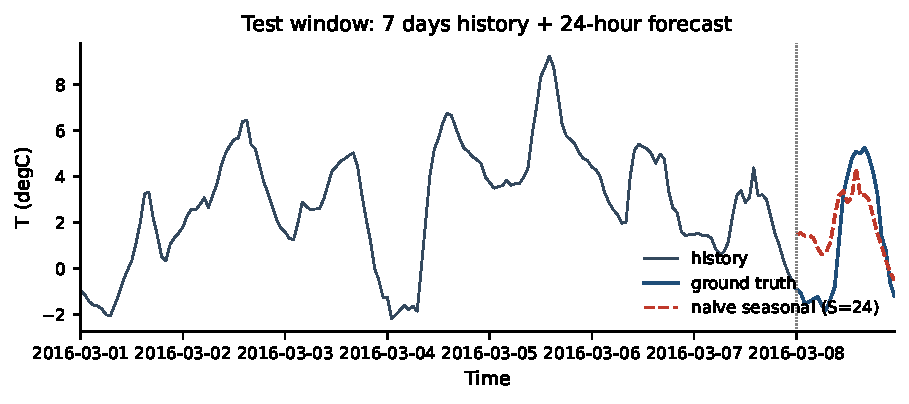
\includegraphics[width=0.86\linewidth]{naive_sample_window.pdf}
\caption{A representative test window from March~2016: seven days of
history, then a 24-hour forecast. The seasonal-naive forecast (red
dashed) shifts the previous day's hourly profile forward. It captures
the diurnal phase almost exactly, but loses day-to-day amplitude
variation, which is the part a learned model is expected to capture.}
\label{fig:naive-window}
\end{figure}

\paragraph{Interpretation of baseline results.}
Naive Seasonal lands at RMSE $3.21$\,$^\circ$C and MAE $2.44$. This is
high but still reasonable for a one-line baseline on a series with a
clear daily cycle. ARIMA$(2,1,2)$ performs worse, with RMSE $4.50$ and
MAE $3.64$. The reason is structural: with $d=1$ and no seasonal
component, ARIMA captures short-range autocorrelation but misses the
24-hour cycle. SARIMA with a seasonal term should reduce this gap, and I
will run it as a control in Phase~2. I keep the plain ARIMA result
because it is a useful negative baseline: it shows that short-range
autocorrelation alone is not enough for this series.

The LSTM beats both classical baselines, reaching RMSE $2.43$
($-24\%$ relative to seasonal naive) and MAE $1.80$ ($-26\%$). Training
and validation losses fall from $0.30/0.22$ at epoch~1 to $0.10/0.11$
at epoch~8, with roughly the same shape on both curves and no late-stage
divergence. The eight-epoch budget appears sufficient for this
preliminary baseline.

\paragraph{Implications for Phase~2.}
The LSTM currently provides the strongest deterministic reference point
at about $2.4$\,$^\circ$C RMSE. A probabilistic model whose predictive
mean is much worse than this reference would need to justify itself
through substantially better uncertainty estimates. Therefore, DeepAR
and the quantile Transformer should be evaluated not only by point
forecasting accuracy, but also by whether their prediction intervals
become more informative under anomalous inputs.

\section{Planned Improvements and Technical Direction}

The next phase will extend the current baseline pipeline in three main directions:

First, I will add two probabilistic forecasters: DeepAR, implemented as an
autoregressive LSTM with a Gaussian or Student-$t$ likelihood and NLL training,
and a quantile-head Transformer trained with pinball loss over a fixed set of
quantiles.

Second, I will extend the current target-only setup by using the
remaining meteorological variables as exogenous covariates, so that the models
can use the full multivariate weather context rather than only past
temperature.

Third, I will evaluate every model under a common anomaly-injection protocol.
The planned anomaly types are point spikes, contextual outliers, level shifts,
and $\ell_{\infty}$-bounded FGSM-style perturbations on the input window.
Probabilistic-specific metrics such as CRPS, pinball loss, prediction-interval
coverage probability (PICP), and mean interval score (MIS) will be added on top
of MAE and RMSE. For relative error reporting, sMAPE and MASE will replace
MAPE. I also plan to add SARIMA$(p,d,q)(P,D,Q)_{24}$ as a control model to
check whether the poor plain-ARIMA result is mainly due to the missing seasonal
component rather than a coding issue.

\section{Ablation and Error Analysis Plan}

\paragraph{Ablation study.}
The ablation study will compare several parts of the pipeline to understand
their contribution. For the input setup, I will compare target-only forecasting
against multivariate forecasting with covariates. For temporal context, I will
test different lookback lengths, such as $L \in \{72, 168, 336\}$. For the
deep models, I will vary hidden capacity and regularization. For DeepAR, I will
compare Gaussian versus Student-$t$ likelihoods. For the quantile Transformer,
I will compare smaller and larger quantile sets, such as 3 versus 7 quantiles.
Finally, I will perform per-anomaly-type ablations to see which injection mode
each model is most sensitive to.

\paragraph{Error analysis.}
The error analysis will examine where and why the models fail. I will break
down MAE/RMSE by forecast horizon to see whether errors grow smoothly or
increase sharply at later hours. I will also compare errors across seasonal
contexts, such as month or temperature range, because winter near-zero
temperatures already caused issues for percentage-based metrics. Under anomaly
injection, the worst failure windows will be grouped by anomaly type and
intensity. For probabilistic models, I will specifically examine
overconfident failures, where the prediction interval is narrow but misses the
true value, because this is the most dangerous failure mode for downstream use.

\section{Visualization and Interpretation Plan}

A first pass is already included in this report:
Figure~\ref{fig:series-split} shows the time series with chronological split
markers, Figure~\ref{fig:summary} compares baseline errors and LSTM training
curves, and Figure~\ref{fig:naive-window} shows a representative 24-hour
forecast window.

In the final phase, I plan to add visualizations that directly support the
main research question. Forecast plots with prediction intervals will show
whether probabilistic models widen their uncertainty around anomalous inputs.
Calibration plots, reliability curves, and PIT histograms will show whether
the predicted uncertainty is statistically meaningful. Per-horizon RMSE and
CRPS curves will show how error changes across the 24-hour forecast horizon.
A model-versus-anomaly heatmap will summarize robustness degradation across
anomaly types and intensities. For the Transformer model, attention maps may
be used as a sanity check to see whether the model attends to
seasonally-aligned positions, although these will be interpreted cautiously
rather than treated as a complete explanation.

\section{GitHub and Reproducibility Status}

\paragraph{Repository.}
The project repository is available at
\url{https://github.com/ozanerdogan/prob-forecast-anomaly}.

\paragraph{Current structure.}
The \texttt{src/} directory contains the main data and modelling code,
including \texttt{data\_loader.py}, \texttt{preprocessing.py},
\texttt{metrics.py}, and the \texttt{src/baselines/} package. The baseline
package currently includes \texttt{naive\_seasonal.py},
\texttt{arima\_baseline.py}, and \texttt{lstm\_baseline.py}.
The \texttt{scripts/} directory contains the runnable entry points:
\texttt{download\_data.py}, \texttt{run\_naive.py},
\texttt{run\_arima.py}, \texttt{run\_lstm.py}, and
\texttt{make\_figures.py}. The \texttt{data/} directory contains
dataset acquisition instructions, while raw and processed data are
gitignored. The \texttt{results/} directory stores JSON metric files
and generated figures, and \texttt{report/} stores the LaTeX source and
compiled report.

\paragraph{Dependencies and README status.}
The repository includes a \texttt{requirements.txt} file for the current
Python environment. It lists the major dependencies used so far,
including \texttt{numpy}, \texttt{pandas}, \texttt{scikit-learn},
\texttt{statsmodels}, \texttt{torch}, \texttt{matplotlib},
\texttt{seaborn}, \texttt{tqdm}, \texttt{pyyaml} and \texttt{pyarrow}. The
\texttt{README.md} documents the current workflow: create a virtual
environment, install dependencies, download and preprocess the dataset,
run the baseline scripts, and regenerate the figures.

\paragraph{Running the current experiments.}
The current pipeline can be reproduced with the following commands:
\begin{verbatim}
python -m venv .venv
source .venv/bin/activate
pip install -r requirements.txt

python scripts/download_data.py
python scripts/run_naive.py
python scripts/run_arima.py
python scripts/run_lstm.py
python scripts/make_figures.py
\end{verbatim}
The dataset preparation step is fully scripted. The raw Jena Climate
archive is downloaded, cleaned, resampled to hourly frequency, and saved
as \texttt{data/processed/jena\_hourly.parquet}. Raw and processed data
are not committed to GitHub.

\paragraph{Reproducibility details.}
Each baseline script writes a JSON file under \texttt{results/} that
contains the evaluation metrics and relevant model configuration. The
LSTM training script uses a fixed random seed with
\texttt{torch.manual\_seed(42)}. This makes the current baseline runs
reasonably reproducible, although small differences may still occur
depending on hardware and PyTorch backend behavior.

\paragraph{Commit history.}
The repository is currently at an early stage, with the initial
baseline pipeline, preprocessing code, figures, and report already
uploaded. The remaining project components will be added through
incremental commits during the final development phase.

\section{Current Challenges and Next Steps}

\paragraph{Current challenges.}
At this stage, computation is manageable, but it may become a constraint in
the next phase. The current LSTM baseline can be trained in a reasonable time,
yet the planned probabilistic models, anomaly-intensity sweeps, and ablation
experiments will require many more training and evaluation runs. For this
reason, I may need to use smaller debugging configurations, limit the number
of repeated runs, or use GPU access for the full final evaluation.

A second challenge is anomaly realism. If anomaly intensity is fixed in
absolute temperature units, the same perturbation may have different meaning
in winter and summer. To make the injected anomalies more comparable across
the year, I plan to scale anomaly intensity using a local rolling standard
deviation. This should make the robustness tests less dependent on the
seasonal temperature level.

A third challenge is probabilistic calibration. Even if a probabilistic model
gives good point forecasts, its nominal prediction intervals may not achieve
the expected empirical coverage. For this reason, validation-set calibration
will be considered in Phase~2, possibly using a simple post-hoc adjustment
such as isotonic calibration or temperature scaling.

\paragraph{Next steps.}
Before the final submission, I plan to complete the probabilistic part of
the pipeline by implementing DeepAR and a quantile-based Transformer. I
will also add SARIMA as a seasonal statistical control, since the current
plain ARIMA baseline performs poorly mainly because it does not model the
24-hour cycle. After that, I will add the anomaly-injection harness with
spikes, contextual outliers, level shifts, and FGSM-style bounded input
perturbations.

The final evaluation will compare deterministic and probabilistic models
on both clean and anomalous test inputs. In addition to MAE and RMSE, I
will report probabilistic metrics such as CRPS, pinball loss, prediction
interval coverage probability (PICP), and mean interval score (MIS). I
will also complete the planned ablation study, error analysis, and
visualizations, then update the final report with the full experimental
results.

\section*{References}

\begin{enumerate}[label={[\arabic*]}]
  \item Rob J. Hyndman and George Athanasopoulos. \emph{Forecasting: Principles and Practice}. 3rd ed. OTexts, 2021. \url{https://otexts.com/fpp3/}

  \item Sepp Hochreiter and J\"{u}rgen Schmidhuber. ``Long Short-Term Memory.'' \emph{Neural Computation}, 9(8):1735--1780, 1997. doi:10.1162/neco.1997.9.8.1735.

  \item David Salinas, Valentin Flunkert, Jan Gasthaus, and Tim Januschowski. ``DeepAR: Probabilistic Forecasting with Autoregressive Recurrent Networks.'' \emph{International Journal of Forecasting}, 36(3):1181--1191, 2020.

  \item Ruofeng Wen, Kari Torkkola, Balakrishnan Narayanaswamy, and Dhruv Madeka. ``A Multi-Horizon Quantile Recurrent Forecaster.'' \emph{arXiv preprint arXiv:1711.11053}, 2017.

  \item Haoyi Zhou, Shanghang Zhang, Jieqi Peng, Shuai Zhang, Jianxin Li, Hui Xiong, and Wancai Zhang. ``Informer: Beyond Efficient Transformer for Long Sequence Time-Series Forecasting.'' \emph{Proceedings of the AAAI Conference on Artificial Intelligence}, 35(12):11106--11115, 2021.

  \item Haixu Wu, Jiehui Xu, Jianmin Wang, and Mingsheng Long. ``Autoformer: Decomposition Transformers with Auto-Correlation for Long-Term Series Forecasting.'' \emph{Advances in Neural Information Processing Systems}, 34:22419--22430, 2021.

  \item Ian J. Goodfellow, Jonathon Shlens, and Christian Szegedy. ``Explaining and Harnessing Adversarial Examples.'' \emph{International Conference on Learning Representations}, 2015.

  \item Aleksander Madry, Aleksandar Makelov, Ludwig Schmidt, Dimitris Tsipras, and Adrian Vladu. ``Towards Deep Learning Models Resistant to Adversarial Attacks.'' \emph{International Conference on Learning Representations}, 2018.

  \item Ane Bl\'{a}zquez-Garc\'{i}a, Angel Conde, Usue Mori, and Jose A. Lozano. ``A Review on Outlier/Anomaly Detection in Time Series Data.'' \emph{ACM Computing Surveys}, 54(3), Article 56, 2021.

  \item Tilmann Gneiting and Adrian E. Raftery. ``Strictly Proper Scoring Rules, Prediction, and Estimation.'' \emph{Journal of the American Statistical Association}, 102(477):359--378, 2007.
\end{enumerate}

\end{document}
